\documentclass[11pt]{article}
\usepackage[margin=25mm]{geometry}
\usepackage{amsmath,amssymb,booktabs,microtype,graphicx}
\usepackage[colorlinks=true,allcolors=blue]{hyperref}
\setlength{\parindent}{0pt}
\setlength{\parskip}{7pt}
\newcommand{\energy}{\mathcal E}
\begin{document}

{\Large\bfseries Which excitatory fraction maximizes the joint dimension?}

\emph{An exact four-coefficient form of $D/N$ along the composition path, the quintic that locates its maximum, when that maximum is unique, and an explicit approximation.}

Along the composition path of the manuscript, the per-neuron dimension of the excitatory population alone falls monotonically with the excitatory fraction, while the total excitatory dimension $D_E/N$ has a maximum at $\sqrt a/(\sqrt a+\sqrt b)$. The joint dimension $D/N$ is also non-monotone, and until now its maximum had only been read off a numerical curve. This note derives it.

The result has four parts. First, within the conditional theory the joint dimension reduces exactly to a ratio with four energy coefficients,
\[
 \frac DN=\frac{\bigl(v_I+(v_E-v_I)f\bigr)^2}{\dfrac{\alpha}{f}+\dfrac{\beta}{1-f}+pf+q(1-f)},
\]
where $f$ is the excitatory fraction. Second, its stationary points in $(0,1)$ are roots of an explicit quintic. For generic coefficients that quintic has no solution in radicals, so the optimum has no closed form in the usual sense; it has closed forms in four special cases, and the inverse question, which variance ratio puts a stationary point at a given fraction, has a closed form. Third, the maximum need not be unique: there are admissible parameters, including solutions of the conditional theory itself, with two local maxima. A simple sufficient condition for uniqueness is given, and the reference parameters are shown to have a single maximum. Fourth, one Newton step from the simplest special case gives an explicit formula that is accurate when the two populations have similar variances and fails when they do not.

For the reference parameters the maximum is at $f^\star=0.851$, with $D/N=0.03466$. The curve is flat there: it stays within $1\%$ of the maximum from $f=0.80$ to $0.89$ and within $0.1\%$ from $0.836$ to $0.865$. The robust predictions are therefore the plateau and the fall on either side, and the third decimal of $f^\star$ is not one of them.

Everything through the section on reference parameters is algebra conditional on the manuscript's closure. Network data enter only in the last two sections: a comparison with the cohorts that existed when the theory was written, and a dedicated experiment of 2{,}920 networks whose design was fixed beforehand. In that experiment the optimum moved with the target rates as predicted and the reference optimum agreed with $0.851$ to within about $0.01$, while the fraction-independence of the underlying coefficients held only up to finite-size errors of up to $12\%$ that shrink with network size.

\textbf{Setup.} There are two populations, $E$ and $I$, with fractions $f_E=f$ and $f_I=g\equiv1-f$. The composition path rescales each presynaptic column of the mean and variance couplings by $f_b^0/f_b$, so that $J^0\,\mathrm{diag}(f)$ and $W=G\,\mathrm{diag}(f)$ stay fixed. Within the theory this leaves the one-site law unchanged, so the mean temporal rate variances $v_E,v_I>0$ do not depend on $f$, and the block covariance energies are
\begin{equation}
 \energy_{ab}(f)=f_af_b\sum_{c\in\{E,I\}}\frac{T_{abc}}{f_c},
 \qquad
 T_{abc}=\int\!\!\int R_{ac}R_{bc}^{*}\,Q_c\,\frac{d\omega_1\,d\omega_2}{(2\pi)^2},
 \label{eq:blocks}
\end{equation}
with a tensor $T_{abc}$ that does not depend on $f$ (manuscript Eq.~(composition)). Here $R=(I-UW)^{-1}$ with $U=H(\omega_1)H(\omega_2)\,\mathrm{diag}(A_a)$ and $H(\omega)=1/(1+i\omega)$, and $Q_c(\omega_1,\omega_2)=\mathbb E_z[c_c(z,\omega_1)c_c(z,\omega_2)]$ is the same-neuron product of conditional spectra. The index $c$ labels the population whose neurons act as sources.

Three properties of $T$ are used.
\begin{itemize}
 \item \emph{It is real.} The integrand is complex at a given frequency pair. Under the reflection $(\omega_1,\omega_2)\to(-\omega_1,-\omega_2)$ we have $H(-\omega)=H(\omega)^*$, so $U\to U^*$ and $R\to R^*$, while $Q_c$ is unchanged because each conditional spectrum is even. The integrand therefore goes to its complex conjugate, and since the integration domain is symmetric under the reflection, the integral equals its own conjugate.
 \item \emph{It is symmetric in its first two indices.} Exchanging $a$ and $b$ replaces $R_{ac}R_{bc}^*$ by its conjugate, so $T_{bac}=T_{abc}^*=T_{abc}$.
 \item \emph{Each source matrix $M_c\equiv[T_{abc}]_{ab}$ is positive semidefinite.} For real $x=(x_E,x_I)$, $\sum_{ab}x_ax_bT_{abc}=\int\!\!\int\bigl|\sum_ax_aR_{ac}\bigr|^2Q_c\ge0$, because the conditional spectra are nonnegative and so is their product averaged over $z$.
\end{itemize}
We assume in addition that $\alpha\equiv T_{IIE}>0$ and $\beta\equiv T_{EEI}>0$, which holds when each population drives the other, and that the total energy is positive on $(0,1)$, which holds when $M_E$ and $M_I$ are positive definite. At the reference parameters their smallest eigenvalues are $0.013$ and $0.0032$.

The joint dimension per neuron is
\begin{equation}
 d(f)\equiv\frac DN=\frac{\nu(f)^2}{\energy(f)},\qquad
 \nu(f)=fv_E+gv_I,\qquad
 \energy(f)=\energy_{EE}+2\energy_{EI}+\energy_{II}.
 \label{eq:d}
\end{equation}
This is the quantity the simulations estimate: same-neuron terms are included in the within-population blocks, the $E$--$I$ block is counted twice, and everything is normalized by the total number of neurons.

\textbf{Step 1: the energy has two poles and a linear remainder.} Insert Eq.~\eqref{eq:blocks} into the total energy and group by source population $c$, using $T_{EIc}=T_{IEc}$:
\begin{align*}
 \energy(f)
 &=\sum_{c}\frac1{f_c}\Bigl[f^2T_{EEc}+2fg\,T_{EIc}+g^2T_{IIc}\Bigr]\\
 &=\frac1f\Bigl[f^2T_{EEE}+2fg\,T_{EIE}+g^2T_{IIE}\Bigr]
  +\frac1g\Bigl[f^2T_{EEI}+2fg\,T_{EII}+g^2T_{III}\Bigr]\\
 &=fT_{EEE}+2g\,T_{EIE}+\frac{g^2}{f}T_{IIE}
  +\frac{f^2}{g}T_{EEI}+2f\,T_{EII}+g\,T_{III}.
\end{align*}
Only two terms are singular on $[0,1]$. Write each as a pole plus a polynomial, using $g=1-f$ and then $1=f+g$:
\begin{align*}
 \frac{g^2}{f}&=\frac{(1-f)^2}{f}=\frac{1-2f+f^2}{f}=\frac1f-2+f=\frac1f-2(f+g)+f=\frac1f-f-2g,\\
 \frac{f^2}{g}&=\frac{(1-g)^2}{g}=\frac{1-2g+g^2}{g}=\frac1g-2+g=\frac1g-2(f+g)+g=\frac1g-2f-g.
\end{align*}
Substituting,
\begin{align*}
 \energy(f)
 &=fT_{EEE}+2g\,T_{EIE}+\Bigl(\frac1f-f-2g\Bigr)T_{IIE}
  +\Bigl(\frac1g-2f-g\Bigr)T_{EEI}+2f\,T_{EII}+g\,T_{III}\\
 &=\frac{T_{IIE}}{f}+\frac{T_{EEI}}{g}
  +f\bigl[T_{EEE}-T_{IIE}-2T_{EEI}+2T_{EII}\bigr]
  +g\bigl[2T_{EIE}-2T_{IIE}-T_{EEI}+T_{III}\bigr].
\end{align*}
Define
\begin{equation}
 \alpha=T_{IIE},\quad\beta=T_{EEI},\quad
 p=T_{EEE}-T_{IIE}-2T_{EEI}+2T_{EII},\quad
 q=2T_{EIE}-2T_{IIE}-T_{EEI}+T_{III}.
 \label{eq:coefficients}
\end{equation}
Then
\begin{equation}
 \boxed{\;\energy(f)=\frac{\alpha}{f}+\frac{\beta}{g}+pf+qg,\qquad
 d(f)=\frac{(fv_E+gv_I)^2}{\dfrac{\alpha}{f}+\dfrac{\beta}{g}+pf+qg}\;}
 \label{eq:reduced}
\end{equation}
The pole at $f=0$ has residue $\alpha=T_{IIE}$, which belongs to the $I$--$I$ covariance generated by excitatory sources: when excitatory cells are rare each of their synapses is strong, and the covariance they induce among the many inhibitory cells diverges as $1/f$. The pole at $f=1$ has residue $\beta=T_{EEI}$, from the $E$--$E$ covariance generated by inhibitory sources. This $\beta$ is the coefficient $b$ in the optimum of $D_E/N$.

Equation~\eqref{eq:reduced} is a partial-fraction form and its four terms are not separate physical contributions: writing $g^2/f$ as $1/f-f-2g$ moved a negative polynomial into the remainder. The coefficients $p$ and $q$ can have either sign. A form that shows their content uses the energy of the difference direction $(1,-1)$ under each source,
\[
 \delta_c\equiv T_{EEc}-2T_{EIc}+T_{IIc}=(1,-1)\,M_c\,(1,-1)^{\!\top}\ge0,\qquad
 k\equiv2\,(T_{EIE}-T_{IIE}+T_{EII}-T_{EEI}).
\]
Adding, $\delta_E+k=T_{EEE}-2T_{EIE}+T_{IIE}+2T_{EIE}-2T_{IIE}+2T_{EII}-2T_{EEI}=T_{EEE}-T_{IIE}-2T_{EEI}+2T_{EII}=p$, and $\delta_I+k=T_{EEI}-2T_{EII}+T_{III}+2T_{EIE}-2T_{IIE}+2T_{EII}-2T_{EEI}=2T_{EIE}-2T_{IIE}-T_{EEI}+T_{III}=q$. Since $f+g=1$,
\[
 \energy(f)=\frac{\alpha}{f}+\frac{\beta}{g}+\delta_Ef+\delta_Ig+k,
 \qquad r\equiv p-q=\delta_E-\delta_I ,
\]
so the slope of the regular part is the difference between the two sources' difference-direction energies.

\textbf{Step 2: the stationarity condition.} Write $\Delta\equiv v_E-v_I$, so that $\nu(f)=v_I+\Delta f$ and $\nu'(f)=\Delta$. Since $dg/df=-1$,
\[
 \frac{d}{df}\frac{\beta}{g}=-\frac{\beta}{g^2}\cdot\frac{dg}{df}=\frac{\beta}{g^2},
 \qquad
 \energy'(f)=-\frac{\alpha}{f^2}+\frac{\beta}{g^2}+p-q=-\frac{\alpha}{f^2}+\frac{\beta}{g^2}+r.
\]
The quotient rule gives
\[
 d'(f)=\frac{2\nu\nu'\energy-\nu^2\energy'}{\energy^2}
      =\frac{\nu\,\bigl(2\Delta\,\energy-\nu\,\energy'\bigr)}{\energy^2}.
\]
On $(0,1)$ both $\nu$ and $\energy$ are positive, so $d'(f)=0$ exactly when
\begin{equation}
 2\Delta\,\energy(f)=\nu(f)\,\energy'(f)
 \quad\Longleftrightarrow\quad
 \frac{\beta}{g^2}-\frac{\alpha}{f^2}=\frac{2\Delta\,\energy(f)}{\nu(f)}-r .
 \label{eq:stationary}
\end{equation}
The left side is the balance between the marginal costs of the two poles. The right side has two corrections: the difference between the two populations' variances, which changes the numerator of $d$ as $f$ moves, and the slope $r$ of the regular part of the energy.

A maximum exists in the open interval. As $f\to0^+$ the energy behaves as $\alpha/f$ and $\nu\to v_I$, so $d\approx v_I^2f/\alpha\to0$. As $f\to1^-$ the energy behaves as $\beta/g$ and $\nu\to v_E$, so $d\approx v_E^2g/\beta\to0$. Since $d$ is continuous and positive inside, it attains a maximum at an interior point, which satisfies Eq.~\eqref{eq:stationary}.

\textbf{Step 3: clearing denominators gives a quintic.} Multiply $\nu\energy'-2\Delta\energy$ by $f^2g^2$. From Eq.~\eqref{eq:reduced},
\begin{align*}
 f^2g^2\,\energy'&=-\alpha g^2+\beta f^2+rf^2g^2,\\
 f^2g^2\,\energy&=\alpha fg^2+\beta f^2g+(pf+qg)f^2g^2 .
\end{align*}
Define
\begin{equation}
 \Phi(f)\equiv f^2g^2\bigl(\nu\energy'-2\Delta\energy\bigr)
 =\nu\,\underbrace{\bigl[\beta f^2-\alpha g^2+rf^2g^2\bigr]}_{B_1}
 -2\Delta\,\underbrace{\bigl[\alpha fg^2+\beta f^2g+(pf+qg)f^2g^2\bigr]}_{B_2},
 \label{eq:phi}
\end{equation}
so that $d'(f)=-\nu\,\Phi(f)/(f^2g^2\energy^2)$ and the stationary points of $d$ in $(0,1)$ are exactly the roots of $\Phi$ there. Now expand in powers of $f$. With $g=1-f$,
\[
 g^2=1-2f+f^2,\qquad fg^2=f-2f^2+f^3,\qquad f^2g=f^2-f^3,\qquad f^2g^2=f^2-2f^3+f^4,
\]
and $pf+qg=pf+q-qf=q+rf$. The first bracket is
\begin{align*}
 B_1&=\beta f^2-\alpha(1-2f+f^2)+r(f^2-2f^3+f^4)\\
    &=-\alpha+2\alpha f+(\beta-\alpha+r)f^2-2rf^3+rf^4 .
\end{align*}
For the second bracket, first
\[
 (q+rf)(f^2-2f^3+f^4)=qf^2-2qf^3+qf^4+rf^3-2rf^4+rf^5
 =qf^2+(r-2q)f^3+(q-2r)f^4+rf^5,
\]
and therefore
\begin{align*}
 B_2&=\alpha(f-2f^2+f^3)+\beta(f^2-f^3)+qf^2+(r-2q)f^3+(q-2r)f^4+rf^5\\
    &=\alpha f+(\beta-2\alpha+q)f^2+(\alpha-\beta+r-2q)f^3+(q-2r)f^4+rf^5 .
\end{align*}
Multiply $B_1$ by $\nu=v_I+\Delta f$:
\begin{align*}
 v_IB_1&=-\alpha v_I+2\alpha v_If+(\beta-\alpha+r)v_If^2-2rv_If^3+rv_If^4,\\
 \Delta fB_1&=-\alpha\Delta f+2\alpha\Delta f^2+(\beta-\alpha+r)\Delta f^3-2r\Delta f^4+r\Delta f^5,
\end{align*}
and $B_2$ by $-2\Delta$:
\[
 -2\Delta B_2=-2\alpha\Delta f-2\Delta(\beta-2\alpha+q)f^2-2\Delta(\alpha-\beta+r-2q)f^3-2\Delta(q-2r)f^4-2r\Delta f^5 .
\]
Collecting each power,
\begin{align*}
 f^0&:\ -\alpha v_I,\\
 f^1&:\ 2\alpha v_I-\alpha\Delta-2\alpha\Delta=\alpha(2v_I-3\Delta),\\
 f^2&:\ (\beta-\alpha+r)v_I+2\alpha\Delta-2\beta\Delta+4\alpha\Delta-2q\Delta=(\beta-\alpha+r)v_I+\Delta(6\alpha-2\beta-2q),\\
 f^3&:\ -2rv_I+(\beta-\alpha+r)\Delta-2\alpha\Delta+2\beta\Delta-2r\Delta+4q\Delta=-2rv_I+\Delta(3\beta-3\alpha-r+4q),\\
 f^4&:\ rv_I-2r\Delta-2q\Delta+4r\Delta=rv_I+\Delta(2r-2q),\\
 f^5&:\ r\Delta-2r\Delta=-r\Delta .
\end{align*}
The stationary points are therefore the roots in $(0,1)$ of
\begin{equation}
 \boxed{\;
 \begin{aligned}
 \Phi(f)={}&-r\Delta\,f^5+\bigl[rv_I+2\Delta(r-q)\bigr]f^4
   +\bigl[-2rv_I+\Delta(3\beta-3\alpha-r+4q)\bigr]f^3\\
  &+\bigl[(\beta-\alpha+r)v_I+2\Delta(3\alpha-\beta-q)\bigr]f^2
   +\alpha(2v_I-3\Delta)f-\alpha v_I=0 .
 \end{aligned}\;}
 \label{eq:quintic}
\end{equation}
Two values check the expansion. At $f=0$, Eq.~\eqref{eq:phi} gives $\Phi(0)=v_I(-\alpha)=-\alpha v_I$, the constant term. At $f=1$ it gives $\Phi(1)=v_E\beta$, and summing the six coefficients, the $v_I$ parts add to $(-\alpha+2\alpha+\beta-\alpha+r-2r+r)v_I=\beta v_I$ and the $\Delta$ parts to $(-3\alpha+6\alpha-2\beta-2q+3\beta-3\alpha-r+4q+2r-2q-r)\Delta=\beta\Delta$, so the sum is $\beta(v_I+\Delta)=\beta v_E$. Since $\Phi(0)<0<\Phi(1)$ and $d'$ has the sign of $-\Phi$, the dimension rises from $f=0$ and falls into $f=1$, consistent with Step 2, and $\Phi$ has an odd number of roots in $(0,1)$ counted with multiplicity.

\textbf{Step 4: when the degree drops.} The leading coefficient is $-r\Delta$.
\begin{itemize}
 \item \emph{Equal variances and flat remainder}, $\Delta=0$ and $r=0$. Only $B_1$ survives and it reduces to $\beta f^2-\alpha g^2=0$. Both $f$ and $g$ are positive, so $\sqrt\beta\,f=\sqrt\alpha\,(1-f)$, that is $f(\sqrt\alpha+\sqrt\beta)=\sqrt\alpha$ and
 \begin{equation}
  f_0=\frac{\sqrt\alpha}{\sqrt\alpha+\sqrt\beta}.
  \label{eq:f0}
 \end{equation}
 This has the same form as the optimum of $D_E/N$, with $T_{IIE}$ in place of $T_{EEE}$.
 \item \emph{Equal variances}, $\Delta=0$, $r\ne0$. Then $\Phi=v_IB_1$ and the condition is the quartic $rf^4-2rf^3+(\beta-\alpha+r)f^2+2\alpha f-\alpha=0$.
 \item \emph{Flat remainder}, $r=0$, $q\Delta\ne0$. The $f^5$ term vanishes and the $f^4$ coefficient becomes $-2q\Delta$, so the condition is again a quartic.
 \item \emph{No regular part}, $p=q=0$, $\Delta(\beta-\alpha)\ne0$. The $f^5$ and $f^4$ coefficients vanish and the condition is the cubic $3\Delta(\beta-\alpha)f^3+\bigl[(\beta-\alpha)v_I+2\Delta(3\alpha-\beta)\bigr]f^2+\alpha(2v_I-3\Delta)f-\alpha v_I=0$.
\end{itemize}
Cubics and quartics are solvable in radicals, so each of these cases has a closed form, although only Eq.~\eqref{eq:f0} is short enough to be useful.

\textbf{Step 5: the general case has no solution in radicals, but the inverse does.} The polynomial $\Phi$ is homogeneous of degree one in $(\alpha,\beta,p,q)$ and in $(v_I,\Delta)$ separately, so its roots depend on four ratios of the six parameters. For six random choices of integer parameters with $\Delta\ne0$ and $r\ne0$, $\Phi$ is irreducible over the rationals and its Galois group is the full symmetric group $S_5$, of order 120, which is not solvable (computed with SymPy; \texttt{check.py}). No root of such a polynomial can be written with rational operations and radicals of its coefficients, so no formula of that kind can hold for all parameters, and a change of variable built from rational operations and radicals cannot help. This does not exclude series, Bring radicals or hypergeometric forms. The exact statement of the optimum is: \emph{$f^\star$ is the root of the quintic \eqref{eq:quintic} in $(0,1)$ at which $d$ is largest.} The restriction to $(0,1)$ matters: at the reference parameters three of the four roots outside the interval have larger $d$ than $f^\star$, and they are not fractions.

The inverse question has an exact closed form, because the stationarity condition \eqref{eq:stationary} is linear in the variances. Writing $2\Delta\energy=(v_I+\Delta f)\energy'$ as $\Delta(2\energy-f\energy')=v_I\energy'$,
\begin{equation}
 \boxed{\;\frac{v_E-v_I}{v_I}=\frac{\energy'(f^\star)}{2\,\energy(f^\star)-f^\star\,\energy'(f^\star)}\;}
 \label{eq:inverse}
\end{equation}
gives the variance difference that places a stationary point at a chosen $f^\star$ for given energy coefficients. Adding one to both sides, $v_E/v_I=(2\energy+g\energy')/(2\energy-f\energy')$ evaluated at $f^\star$, which is an admissible answer only where this ratio is positive. For the reference energy coefficients that is the range $0.306\le f^\star\le0.935$; outside it no pair of positive variances has a stationary point at $f^\star$.

\textbf{Step 6: the maximum is not always unique.} Step 3 allows one, three or five roots in $(0,1)$. Three do occur. With $(\alpha,\beta,p,q,v_E,v_I)=(0.001,0.001,8.997,0.997,3,1)$, which corresponds to $T_{EEE}=9$, $T_{III}=1$, $T_{EIE}=T_{EII}=0$ and has positive energy throughout, $\Phi$ has roots $0.0172$, $0.2481$ and $0.9843$ with $d=0.896$, $0.749$ and $0.986$: two local maxima separated by a minimum. The same happens inside the conditional theory. For aggregate variance couplings $W=\bigl(\begin{smallmatrix}21.769&0.1731\\0.184&35.9971\end{smallmatrix}\bigr)$ and target rates $(0.2615,0.0809)$, the conditional solution gives $\alpha=5.2\times10^{-5}$, $\beta=8.3\times10^{-6}$, $p=0.540$, $q=0.026$, $v_E=0.172$, $v_I=0.035$, and $\Phi$ has roots $0.0148$, $0.1505$ and $0.9951$ with $d=0.0369$, $0.0300$ and $0.0547$. Both examples have weak cross-coupling, so the poles are weak, and very unequal variances. They are statements about the leading theory: the outer maxima lie within $0.02$ of the ends, where the density condition of the Scope section demands very large networks.

A sufficient condition for uniqueness follows from a change of variables that makes $1/d$ a sum of convex terms. Put
\[
 u\equiv\frac f\nu,\qquad w\equiv\frac g\nu .
\]
Then $v_Eu+v_Iw=(v_Ef+v_Ig)/\nu=1$ and $u+w=(f+g)/\nu=1/\nu$. The map $f\mapsto(u,w)$ is monotone, since $du/df=(\nu-f\nu')/\nu^2=(v_I+\Delta f-f\Delta)/\nu^2=v_I/\nu^2>0$, and it carries $(0,1)$ onto the open segment of the line $v_Eu+v_Iw=1$ in the positive quadrant. Stationary points of $d$ in $f$ are therefore stationary points of $1/d$ along that segment. Substituting $f=u\nu$, $g=w\nu$ and then $1/\nu=u+w$,
\begin{align*}
 \frac1d=\frac{\energy}{\nu^2}
 &=\frac1{\nu^2}\Bigl[\frac{\alpha}{u\nu}+\frac{\beta}{w\nu}+pu\nu+qw\nu\Bigr]
  =\frac{\alpha}{u\nu^3}+\frac{\beta}{w\nu^3}+\frac{pu+qw}{\nu}\\
 &=\alpha\,\frac{(u+w)^3}{u}+\beta\,\frac{(u+w)^3}{w}+(pu+qw)(u+w).
\end{align*}
The function $\psi(s,u)=s^3/u$ has second derivatives $\psi_{ss}=6s/u$, $\psi_{su}=-3s^2/u^2$ and $\psi_{uu}=2s^3/u^3$, so its Hessian has determinant $12s^4/u^4-9s^4/u^4=3s^4/u^4>0$ and positive trace for $s,u>0$. It is strictly convex, and so is $(u+w)^3/u$, which is $\psi$ composed with the invertible linear map $(u,w)\mapsto(u+w,u)$. The same holds for $(u+w)^3/w$. The last term is the quadratic form $pu^2+(p+q)uw+qw^2$, whose second derivative along the segment direction $\tau=(v_I,-v_E)$ is
\[
 2\bigl[pv_I^2-(p+q)v_Iv_E+qv_E^2\bigr]=2\,(pv_I-qv_E)(v_I-v_E)=-2\Delta\,(pv_I-qv_E).
\]
Hence
\begin{equation}
 \boxed{\;\Delta\,(pv_I-qv_E)\le0\ \Longrightarrow\ \text{$d$ has exactly one stationary point in $(0,1)$,}\;}
 \label{eq:unique}
\end{equation}
because $1/d$ is then strictly convex along the segment, and a strictly convex function has at most one stationary point, which Step 2 shows exists. More generally the conclusion holds whenever the convex pole terms outweigh the quadratic term everywhere on the segment. Both counterexamples violate \eqref{eq:unique}, with $\Delta(pv_I-qv_E)=12.0$ and $0.0020$.

\textbf{Step 7: an explicit approximation and its range.} Write Eq.~\eqref{eq:stationary} as $\Psi(f)\equiv h(f)-\kappa(f)=0$ with
\[
 h(f)=\frac{\beta}{g^2}-\frac{\alpha}{f^2},\qquad
 \kappa(f)=\frac{2\Delta\,\energy(f)}{\nu(f)}-r .
\]
Comparing with Eq.~\eqref{eq:phi}, $\Phi=f^2g^2\nu\,(\energy'-2\Delta\energy/\nu)=f^2g^2\nu\,(h+r-2\Delta\energy/\nu)=f^2g^2\nu\,\Psi$, so $d'$ has the sign of $-\Psi$. By construction $h(f_0)=0$ at the point $f_0$ of Eq.~\eqref{eq:f0}, so $\Psi(f_0)=-\kappa(f_0)$ and $d'(f_0)$ has the sign of $\kappa(f_0)$. When the stationary point is unique this gives an exact statement about direction:
\[
 \operatorname{sign}(f^\star-f_0)=\operatorname{sign}\Bigl(\frac{2\Delta\,\energy(f_0)}{\nu(f_0)}-r\Bigr).
\]
One Newton step from $f_0$ is $f_1=f_0-\Psi(f_0)/\Psi'(f_0)=f_0+\kappa(f_0)/\bigl(h'(f_0)-\kappa'(f_0)\bigr)$. Each ingredient is explicit. Let $s\equiv\sqrt\alpha+\sqrt\beta$, so that $f_0=\sqrt\alpha/s$ and $g_0=\sqrt\beta/s$. Then
\begin{align*}
 h'(f)&=\frac{d}{df}\bigl[\beta g^{-2}-\alpha f^{-2}\bigr]=\frac{2\beta}{g^3}+\frac{2\alpha}{f^3},\\
 h'(f_0)&=\frac{2\beta s^3}{\beta^{3/2}}+\frac{2\alpha s^3}{\alpha^{3/2}}
  =2s^3\Bigl(\frac1{\sqrt\beta}+\frac1{\sqrt\alpha}\Bigr)
  =2s^3\,\frac{\sqrt\alpha+\sqrt\beta}{\sqrt{\alpha\beta}}
  =\frac{2s^4}{\sqrt{\alpha\beta}},\\
 \energy_0\equiv\energy(f_0)&=\frac{\alpha s}{\sqrt\alpha}+\frac{\beta s}{\sqrt\beta}+\frac{p\sqrt\alpha+q\sqrt\beta}{s}
  =s\bigl(\sqrt\alpha+\sqrt\beta\bigr)+\frac{p\sqrt\alpha+q\sqrt\beta}{s}
  =s^2+\frac{p\sqrt\alpha+q\sqrt\beta}{s},\\
 \nu_0\equiv\nu(f_0)&=\frac{v_E\sqrt\alpha+v_I\sqrt\beta}{s}.
\end{align*}
For the derivative of $\kappa$, the quotient rule gives $\kappa'=2\Delta(\energy'\nu-\energy\Delta)/\nu^2$, and at $f_0$ the energy slope is $\energy'(f_0)=h(f_0)+r=r$. Hence
\begin{equation}
 \boxed{\;
 f^\star\approx f_1=\frac{\sqrt\alpha}{s}
 +\frac{\dfrac{2\Delta\,\energy_0}{\nu_0}-r}
       {\dfrac{2s^4}{\sqrt{\alpha\beta}}-\dfrac{2\Delta\,(r\nu_0-\Delta\,\energy_0)}{\nu_0^2}},
 \qquad s=\sqrt\alpha+\sqrt\beta .\;}
 \label{eq:newton}
\end{equation}
This is one step of an iteration and carries no error bound. It is useful when the step is small compared with the distance from $f_0$ to the nearer endpoint, that is when
$\epsilon\equiv|\kappa(f_0)|/\bigl[h'(f_0)\min(f_0,g_0)\bigr]\ll1$, and when $h'(f_0)-\kappa'(f_0)>0$. Table~\ref{tab:newton} shows how it degrades with the variance difference, at the reference couplings with unequal target rates. In the conditional-theory counterexample of Step 6, $\epsilon\approx10^{3}$, the denominator is negative, and the step leaves the interval.

\begin{table}[h]
\centering
\begin{tabular}{lrrrrr}
\toprule
target rates $(E,I)$ & $f^\star$ & $f_0$ & $f_1$ & $\epsilon$ & loss of $d$ at $f_1$\\
\midrule
$(0.30,0.30)$ reference & 0.8510 & 0.8737 & 0.8553 & 0.15 & $0.009\%$\\
$(0.15,0.15)$ & 0.8307 & 0.8729 & 0.8432 & 0.24 & $0.07\%$\\
$(0.25,0.35)$ & 0.8221 & 0.8879 & 0.8505 & 0.34 & $0.36\%$\\
$(0.20,0.40)$ & 0.7866 & 0.9017 & 0.8562 & 0.48 & $2.2\%$\\
$(0.10,0.50)$ & 0.6940 & 0.9308 & 0.8864 & 0.77 & $22\%$\\
$(0.50,0.10)$ & 0.9300 & 0.7869 & 1.3768 & 3.3 & outside $(0,1)$\\
\bottomrule
\end{tabular}
\caption{Exact optimum, the special-case point $f_0$ and the one-step formula \eqref{eq:newton} for the reference couplings at several target rates. Each row has a single stationary point in $(0,1)$. The optimum itself moves from $0.69$ to $0.93$ across these rates.}
\label{tab:newton}
\end{table}

\textbf{Reference parameters.} For the manuscript's reference couplings at Bernoulli dispersion and target rates $0.3$, \texttt{check.py} evaluates the tensor from the conditional solution and gives the values in Table~\ref{tab:values}. The imaginary part of the integrated tensor is below $10^{-16}$.

\begin{table}[h]
\centering
\begin{tabular}{llll}
\toprule
$T_{EEE}=0.4800$ & $T_{EIE}=0.4079$ & $T_{IIE}=0.3698$ & $v_E=0.14396$\\
$T_{EEI}=0.00772$ & $T_{EII}=0.02034$ & $T_{III}=0.09498$ & $v_I=0.16637$\\
\midrule
$\alpha=0.36978$ & $\beta=0.007722$ & $p=0.13546$ & $q=0.16348$\\
$\delta_E=0.03400$ & $\delta_I=0.06202$ & $k=0.10146$ & \\
$r=-0.02802$ & $\Delta=-0.02241$ & & \\
\bottomrule
\end{tabular}
\caption{Fraction-independent inputs at the reference parameters and the coefficients of Eq.~\eqref{eq:coefficients}.}
\label{tab:values}
\end{table}

The quintic \eqref{eq:quintic} has roots $-5.655$, $0.8510$, $1.232$, $2.157$ and $7.660$. The only one in $(0,1)$ is
\[
 f^\star=0.8510,\qquad d(f^\star)=0.034659,\qquad \nu=0.14729,\qquad \energy=0.6260,
\]
and a direct search over two million values of $f$ returns the same maximum. Changing the lag step, the horizon, the number of Hermite nodes and the frequency cutoff of the quadrature moves $f^\star$ by less than $10^{-8}$. Equation~\eqref{eq:inverse} evaluated at $f^\star$ returns $\Delta/v_I=-0.13472$, the input value.

The maximum is unique here, but not by the sufficient condition: $\Delta(pv_I-qv_E)=+2.2\times10^{-5}$, so the quadratic term is slightly concave along the segment. Its curvature per unit length is $-0.0009$, against a total curvature of $1/d$ that is at least $1.17$ on the segment (the minimum, $1.176$, is near $f=0.72$, and the pole terms diverge toward both ends), so $1/d$ is strictly convex and the root count of one is confirmed.

By block and source, the energy at the optimum is: $E$--$E$ from $E$ sources $0.4085$; $E$--$I$ (counted twice) from $E$ sources $0.1215$; $E$--$E$ from $I$ sources $0.0375$; $E$--$I$ from $I$ sources $0.0346$; $I$--$I$ from $I$ sources $0.0141$; $I$--$I$ from $E$ sources $0.0096$. The two cross-driven terms that carry the poles are $7.5\%$ of the energy at the optimum. They set the location of the maximum through their steep dependence on $f$, while most of the energy is excitatory covariance from excitatory sources.

The special-case point is $f_0=0.8737$, where $d$ is $0.27\%$ below its maximum. In Eq.~\eqref{eq:newton} the numerator is $2\Delta\energy_0/\nu_0-r=-0.190+0.028=-0.162$ and the denominator is $8.781+0.021$, giving $f_1=0.8553$, which is $0.0042$ above $f^\star$ and loses $0.009\%$ of the maximum. A second Newton step gives $0.8512$. The variance difference accounts for nearly all of the shift from $f_0$: with $\Delta$ set to zero the optimum is $0.877$.

Three features decide how this result can be used. First, the joint optimum lies below the optimum of total excitatory dimension, $0.8874$, where $d$ is $0.78\%$ below its maximum. Second, the maximum is shallow: the relative curvature is $d''/d=-9.3$, so $d$ is within $1\%$ of its maximum for $f$ between $0.799$ and $0.892$ and within $0.1\%$ between $0.836$ and $0.865$, while the flanks are steep, $d(0.6)=0.02989$ and $d(0.94)=0.03203$. Third, the location is sensitive to the one-site variances: raising $v_E$ by $5\%$ moves $f^\star$ by $+0.010$, and raising $v_I$ by $5\%$ moves it by $-0.013$.

\textbf{Comparison with simulated networks.} Two cohorts of 2{,}000-neuron networks exist. The theory is a large-$N$ statement and these networks are not at the limit, so each comparison below carries a finite-size offset in $D/N$: about $1\%$ near the peak and up to $9\%$ at the low-fraction end.

\emph{Thirteen fractions, 48 networks each} (the paper campaign). The cell means lie between $0.91$ and $1.04$ of the prediction. They are not statistically consistent with it: $\chi^2=51$ on 13 cells, driven by $f=0.65$ ($4.9$ standard errors low) and $f=0.50$ ($3.2$ low). At this size the measured rate variance is $0.99$ to $1.06$ of its prediction and the energy $1.03$ to $1.14$, with partial cancellation in the ratio, and the mean of per-network ratios exceeds the ratio of means by 0.6 to 2.8\%; the manuscript's ratio-bias identity requires the sign. The largest cell mean, $0.0359\pm0.0006$ at $f=0.86$, is $1.9$ standard errors above the prediction with its neighbours at $-0.6$ and $+0.4$, so it carries no information about where the maximum is. The seed-paired changes from $f=0.80$ resolve both flanks: $-0.0051$ at $0.60$ (95\% interval $-0.0069$ to $-0.0033$; predicted $-0.0044$) and $-0.0016$ at $0.94$ ($-0.0031$ to $-0.00004$; predicted $-0.0023$). The seed matching buys no precision, since the networks at different fractions are regenerated: the paired differences have about $\sqrt2$ times the single-network spread.

\emph{Three fractions, 624 networks each} (the readout confirmation; estimator window of 8{,}000 leak times with no gap). Joint $D/N$ was not one of that experiment's prespecified endpoints, so the contrasts here are post hoc. The cell means of the joint $D/N$ are $0.03370\pm0.00019$, $0.03424\pm0.00018$ and $0.03158\pm0.00017$ at $f=0.80$, $0.88$ and $0.94$, which are $0.982$, $0.992$ and $0.986$ of the predictions. The paired change is $+0.00053$ from $0.80$ to $0.88$ (95\% interval $+0.00003$ to $+0.00103$; predicted $+0.00017$) and $-0.00266$ from $0.88$ to $0.94$ ($-0.00314$ to $-0.00217$; predicted $-0.00247$). So $D/N$ is marginally higher at $0.88$ than at $0.80$ ($p=0.04$) and falls clearly by $0.94$, with both predicted changes inside their intervals.

\emph{What would locate the maximum.} Three fractions cannot locate a maximum without assuming the shape of the curve. A model-free comparison of $f=0.851$ with $0.887$ has to resolve a predicted difference of $0.78\%$. With a single-network spread of $0.0047$ at $N=2{,}000$ that takes about 4{,}800 networks per fraction for 80\% power at the 5\% level, which is feasible. Sample size may not be the only constraint, however. Near the peak the finite-size offset is about $1.3\%$ (a common factor of $0.987$ fits the three triplet means, $\chi^2=1.9$ on 2 degrees of freedom), and its variation between $f=0.80$ and $0.88$ is constrained only to $+1.05\pm0.77$ percentage points, which is the size of the effect. Over the whole path the offset does vary: after one common factor the thirteen cell means of the sweep still give $\chi^2=35.9$ on 12 degrees of freedom, although restricted to $f\ge0.80$ this is $8.6$ on 6. A two-point comparison at $N=2{,}000$ therefore cannot be read as a test of the theory until that variation is bounded. This points to either larger networks, where both the offset and the spread are smaller, or a comparison that goes through the structure of the theory: estimate the six coefficients $T_{abc}$ from the measured block energies by the linear relation \eqref{eq:blocks}, compare them with their predicted values, and compute the optimum from the measured coefficients and variances.

\textbf{A dedicated test.} The comparison through the structure of the theory was then run as a separate experiment, with its design, predictions and decision rules written down before any of its networks was simulated (\texttt{validation/EXPERIMENT.md}; results in \texttt{validation/README.md}). It used 2{,}920 new networks on the composition path at ten fractions from $0.60$ to $0.94$ and three pairs of target rates $(m_E,m_I)$: the reference $(0.3,0.3)$, and $(0.2,0.4)$ and $(0.4,0.2)$, for which the theory predicts optima at $0.787$ and $0.895$. Sizes were $N=2{,}000$ (64 networks per fraction), $4{,}000$ and $8{,}000$ (16 each), and $16{,}000$ for the reference rates only (4 each). For each rate pair and size the six coefficients $T_{abc}$ were fitted to the measured block energies with the linear forms of Step 1, $v_a$ was taken as the mean measured rate variance, and the optimum was computed from these by the quintic \eqref{eq:quintic}. Intervals are 95\% bootstrap intervals over networks.

\begin{table}[h]
\centering\small\setlength{\tabcolsep}{4pt}
\begin{tabular}{lccccc}
\toprule
rates & theory & $N=2{,}000$ & $4{,}000$ & $8{,}000$ & $16{,}000$\\
\midrule
$(0.3,0.3)$ & 0.851 & 0.862 [0.848, 0.878] & 0.852 [0.838, 0.868] & 0.851 [0.841, 0.861] & 0.839 [0.826, 0.853]\\
$(0.2,0.4)$ & 0.787 & 0.791 [0.778, 0.803] & 0.789 [0.774, 0.804] & 0.784 [0.774, 0.793] & \\
$(0.4,0.2)$ & 0.895 & 0.893 [0.877, 0.912] & 0.891 [0.871, 0.914] & 0.903 [0.890, 0.918] & \\
\bottomrule
\end{tabular}
\caption{Optimum computed from fitted coefficients and measured variances, with 95\% bootstrap intervals. An independent refit of the per-network table reproduces every entry to within $0.001$.}
\label{tab:validation}
\end{table}

\begin{figure}[h]
\centering
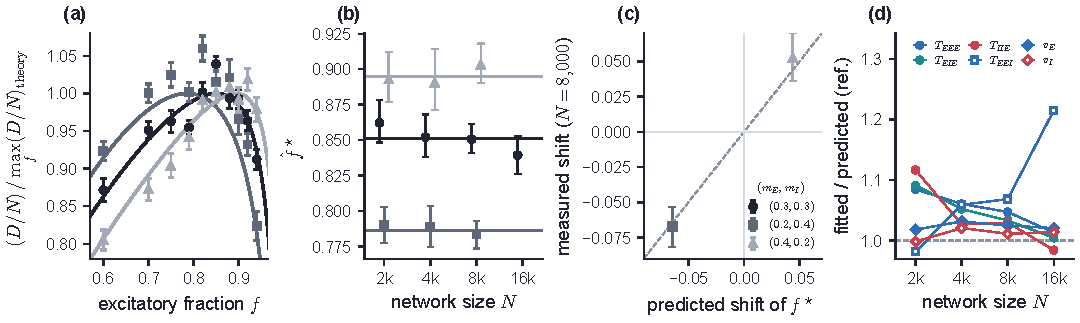
\includegraphics[width=\linewidth]{validation/figures/paper_composition_optimum.pdf}
\caption{(a) $D/N$ against excitatory fraction at $N=8{,}000$ for the three rate pairs, each divided by the maximum of its parameter-only curve (lines); markers are ratios of cell means with one standard error. (b) Optimum computed from the fitted structure against network size, with 95\% bootstrap intervals; lines are the predictions $0.851$, $0.787$ and $0.895$. (c) Shift of the fitted optimum from the reference rates at $N=8{,}000$ against the predicted shift. (d) Fitted coefficients over predicted at the reference rates against size; $T_{EEI}$, the residue $\beta$, is poorly determined.}
\label{fig:validation}
\end{figure}

Three outcomes follow, judged by the rules fixed in advance.
\begin{itemize}
 \item \emph{The optimum moves with the target rates as predicted.} At $N=8{,}000$ the shift from the reference to $(0.2,0.4)$ is $-0.067$ $[-0.082,-0.053]$ against a predicted $-0.064$, and to $(0.4,0.2)$ it is $+0.053$ $[+0.036,+0.070]$ against $+0.044$. Both intervals exclude zero and contain the prediction, at all three sizes. A model-free contrast, the change in $\log D/N$ between $f=0.70$ and $0.94$ relative to the reference, has the predicted sign at every size and at $N=8{,}000$ is $-0.153$ $[-0.215,-0.091]$ and $+0.157$ $[+0.099,+0.214]$ against $-0.167$ and $+0.106$.
 \item \emph{The reference optimum is consistent with $0.851$ and below $0.887$.} The interval contains $0.851$ and excludes $0.887$ at both $8{,}000$ and $16{,}000$ neurons, and every bootstrap draw in every cohort has a single interior maximum. The estimate drifts downward with size, from $0.862$ to $0.839$, and the $16{,}000$-neuron point rests on four networks per fraction, so whether the large-$N$ value is $0.851$ or about $0.01$ lower is not resolved.
 \item \emph{The fraction-independent structure holds only up to finite-size error.} The pre-set criterion, every influential fitted coefficient within $10\%$ of its prediction at the largest size, was not met. At $(0.2,0.4)$ the fitted $T_{EEE}$ is $12\%$ above prediction at $N=8{,}000$, down from $27\%$ at $2{,}000$, and $v_E$ is $8\%$ above. At the reference rates the large coefficients are within $1.5\%$ at $16{,}000$ neurons, and only the small residue $T_{EEI}$, which is poorly determined, deviates. The agreement of the optimum at $(0.2,0.4)$ is therefore partly a cancellation: the fitted coefficients with predicted variances give $0.771$, the predicted coefficients with measured variances give $0.799$, and together they give $0.784$.
\end{itemize}
The estimate of the optimum is model-based throughout: it assumes the block forms of Step 1, which fit the cell means within their noise at $N\ge4{,}000$. Ten of the 2{,}920 networks, all at rates $(0.4,0.2)$ and $N=2{,}000$, ended at a fixed point and are excluded.

\textbf{Scope.} The reduction \eqref{eq:reduced}, the quintic \eqref{eq:quintic}, the inverse \eqref{eq:inverse} and the uniqueness condition \eqref{eq:unique} are exact consequences of Eq.~\eqref{eq:blocks}. They inherit its assumptions: the leading-order closure, and a path on which $J^0\,\mathrm{diag}(f)$ and $G\,\mathrm{diag}(f)$ are held fixed so that the one-site law does not move. On a path that holds individual edge moments fixed instead, $v_a$ and $T_{abc}$ depend on $f$ and none of this applies without a new calculation. The algebra does not require equal target rates, but the optimum depends strongly on them (Table~\ref{tab:newton}).

The path also has a density condition near its ends. The connection probabilities are $p_{ab}=s_bJ^{0\,2}_{ab}/(G_{ab}+s_bJ^{0\,2}_{ab})$ with $s_b=f_b^0/f_b$, which stay in $(0,1)$ but approach one as $f_b\to0$. The number of absent $I\to I$ edges per row is $Ng^2G_{II}/(gG_{II}+f_I^0J^{0\,2}_{II})$, which at $N=2{,}000$ is $24$ at $f^\star$, $11$ at $f=0.90$, $4.2$ at $0.94$ and $1.1$ at $0.97$. The pole $\beta/g$ that produces the downturn is therefore tested, at this size, where the disorder contributed by inhibitory sources comes from a handful of missing edges. The leading theory needs $Ng^2\gg1.7$ there, which is a stronger requirement than a large inhibitory population.

The optimum is a property of covariance geometry on this path and carries no statement about function.

\end{document}
